% -*- TeX-master: "main"; fill-column: 72 -*-

\newcommand{\fixttspace}{\hspace*{1pt}}

\section{Package syntax and semantics}
\label{sec:syntax}

In this section, we define the syntax and semantics of the Hierarchical
Model Composition package for \sbmlthreecore.  We expound on the
various data types and constructs defined in this package, then in
\sec{examples}, we provide complete examples of using the constructs in
example SBML models.

% -----------------------------------------------------------------------------
\subsection{Namespace URI and other declarations necessary for using this package}
\label{xml-namespace}

Every SBML Level~3 package is identified uniquely by an XML namespace
URI.  For an SBML document to be able to use a given Level~3
package, it must declare the use of that package by referencing its URI.
The following is the namespace URI for this version of the Hierarchical
Model Composition package for \sbmlthreecore:
\begin{center}
\uri{http://www.sbml.org/sbml/level3/version1/comp/version1}
\end{center}

In addition, SBML documents using a given package must indicate whether
understanding the package is required for complete mathematical
interpretation of a model, or whether the package is optional.  This is
done using the attribute \token{required} on the \token{<sbml>} element
in the SBML document.  For the Hierarchical Model Composition package,
the value of this attribute may be set to \val{true} or \val{false},
depending on whether the constructs described in this package are used
in the model to change its mathematical meaning.

The following fragment illustrates the beginning of a typical SBML model
using \sbmlthreecore and this version of the Hierarchical Model
Composition package:

\begin{example}
<?xml version="1.0" encoding="UTF-8"?>
<sbml xmlns="http://www.sbml.org/sbml/level3/version1/core" level="3" version="1"
      xmlns:comp="http://www.sbml.org/sbml/level3/version1/comp/version1" comp:required="true">
\end{example}
    

% -----------------------------------------------------------------------------
\subsection{Primitive data types}
\label{new-primitive-types}

Section~3.1 of the \sbmlthreecore specification defines a number of
primitive data types and also uses a number of XML Schema 1.0 data
types~\citep{biron:2000}.  We assume and use some of them in the rest of
this specification, specifically \primtype{boolean}, \primtype{ID},
\primtype{SId}, \primtype{SIdRef}, \primtype{UnitSId},
\primtype{UnitSIdRef}, and \primtype{string}.  The Hierarchical Model
Composition package also makes use of or defines other primitive types;
they are described below.


\subsubsection{Type \fixttspace\primtypeNC{IDREF}}
\label{primtype-idref}

Type \primtype{IDREF} is defined by XML Schema 1.0.  It is a character
string data type whose value is identical to an \primtype{ID} defined 
elsewhere in a referenced document, and has identical syntax.


\subsubsection{Type \fixttspace\primtypeNC{anyURI}}
\label{primtype-anyuri}
\label{primtype-uri}

Type \primtype{anyURI} is defined by XML Schema 1.0.  It is a character
string data type whose values are interpretable as URIs (\emph{Universal
  Resource Identifiers}; \citealt{harold:2001,w3c:2000}) as described by
the W3C document RFC~3986~\citep{rfc3986}.


\subsubsection{Type \fixttspace\primtypeNC{PortSId}}
\label{primtype-portid}

The type \primtype{PortSId} is derived from \primtype{SId}
(\sbmlthreecore specification Section~3.1.7) and has identical syntax.
The \primtype{PortSId} type is used as the data type for the identifiers
of \Port objects (see \sec{port-class}) in the Hierarchical Model
Composition package.  The purpose of having a separate type for such
identifiers is to enable the space of possible port identifier values to
be separated from the space of all other identifier values in SBML.  The
equality of \primtype{PortSId} values is determined by an exact
character sequence match; i.e., comparisons of these identifiers must be
performed in a case-sensitive manner.


\subsubsection{Type \fixttspace\primtypeNC{PortSIdRef}}
\label{primtype-portidref}

Type \primtype{PortSIdRef} is used for all attributes that refer to
identifiers of type \primtype{PortSId}.  This type is derived from
\primtype{PortSId}, but with the restriction that the value of an
attribute having type \primtype{PortSIdRef} must match the value of a
\primtype{PortSId} attribute in the relevant model;  in other words, the value of
the attribute must be an existing port identifier in
the referenced model.  As with \primtype{PortSId}, the equality of
\primtype{PortSIdRef} values is determined by exact character sequence
match; i.e., comparisons of these identifiers must be performed in a
case-sensitive manner.


% -----------------------------------------------------------------------------
\subsection{The extended \class{SBML} class}
\label{sbml-class}
\label{listofmodeldefinitions-class}
\label{listofexternalmodeldefinitions-class}

The top level of an ``SBML document'' is a container whose structure is
defined by the object class \SBML in the \sbmlthreecore specification.  In
Level~3 Core, this container can contain only one model, an object of
class \Model.  The Hierarchical Model Composition package allows SBML
documents to contain \emph{more} than one model.

To explain how this is accomplished, we first need to introduce some
terminology.  In the approach taken here, we make a distinction between
(a) the definition of a model, before it is actually used anywhere, and
(b) its actual use:

\begin{itemize}

\item The term \emph{model definition} refers to the former case; that
  is, the definition of a model, before it is used.  A model definition
  is akin to a Platonic ideal: it may be a complete model in and of
  itself, but until it is instantiated, it exists only as a concept.

\item The term \emph{submodel} refers to actual use of a model
  definition.  A submodel is an instantiation or instance of a
  previously-defined model: it is the realization of that model inside
  another model.  From the perspective of the model that contains this
  submodel, the model definition has come into being, and now exists as
  something that can be used (and possibly modified and adapted).

\end{itemize}

% [MH] Took this out because it wasn't clear that it was needed:
% 
% The potentially arbitrary nesting possible in model composition adds an
% additional wrinkle to the model definition/submodel distinction.  If the
% model directly containing a given submodel is the \Model object of the
% SBML document, then the submodel has been fully instantiated.  However,
% if the containing model is instead \emph{another} model definition (call
% it ``M''), the submodel becomes part of that larger model definition,
% but has \emph{not} been fully instantiated in the SBML document.  The
% submodel only becomes fully instantiated when the model definition
% (``M'') is itself instantiated in the top-level \Model object of an SBML
% document.

It may be helpful to contrast these terms with those in other
approaches to model composition.  Some approaches call the model
definitions themselves the ``submodels''.  We avoid that usage because,
in the present formulation, model definitions must be valid \Model
objects in and of themselves, and might never appear inside other models
in the SBML document where they are defined.  (This might be the
situation, for example, if the document defines multiple models purely
to serve as a sort of component library used by other files.)  We
reserve the term ``submodel'' specifically for the \emph{instance of a
  model inside a containing model}.  Another term used in other schemes
is ``model template'', which is close to what is intended by ``model
definition'' here, but ``template'' implies something that is incomplete
and needs to be filled in.  While this is possible in the approach
described here, it is not required; for example, in model aggregation,
several complete working models may be integrated to form a larger
whole.  We therefore eschew the term ``model template'' in favor of
\emph{model definition}.

\begin{figure}[b]
  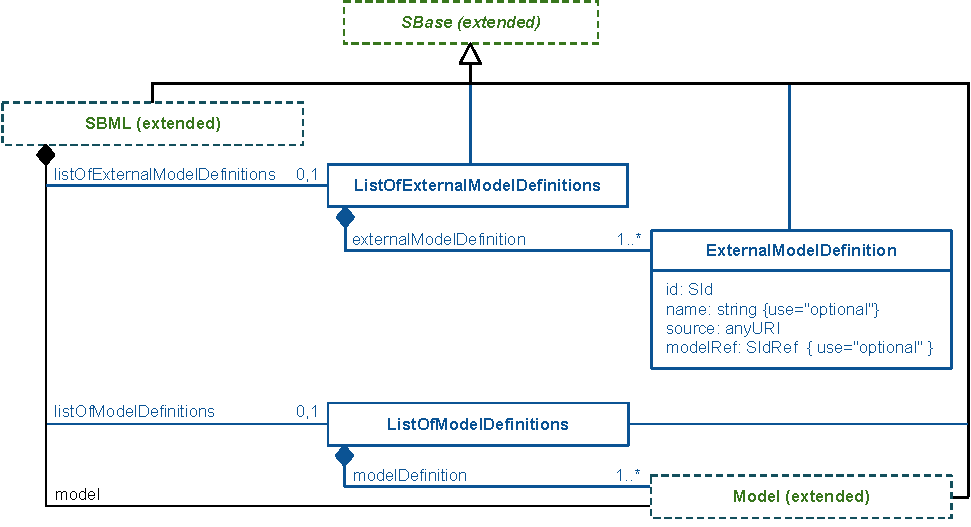
\includegraphics{figs/hierarchical-sbml}
  \caption{The definitions of the extended \SBML class as well as the
    new classes \ListOfModelDefinitions,
    \ListOfExternalModelDefinitions, and \ExternalModelDefinition.  The
    extended \Model class is defined in \sec{model-class}.}
  \label{hierarchical-sbml-uml}
  \label{sbml-uml}
\end{figure}

\fig{hierarchical-sbml-uml} gives the definition of the extended \SBML
class. It ties these different components together and also provides the
definition of \ExternalModelDefinition.  Readers familiar with the \SBML
class in \sbmlthreecore will notice that the Hierarchical Model
Composition package adds two new lists to \SBML:
\token{listOfModelDefinitions} of class \ListOfModelDefinitions and
\token{listOfExternalModelDefinitions} of class
\ListOfExternalModelDefinitions.  The class diagram also makes concrete
the notions described above, that model definition objects are not
``owned'' by any other model (they can be instantiated anywhere, even by
models in other files) and that they exist outside the \Model class
entirely.

\fig*{hierarchical-sbml-uml} also makes clear how model definitions
\emph{are} \Model objects.  At the same time, the scheme preserves the
aspect of \sbmlthreecore in which a single \Model object appears at the
top level of an SBML document.  As will become clear when we define
\Model, submodels appear inside \Model objects.  This is a crucial
feature of the design described above; namely, when the top-level model
references submodels, the submodels are instantiated, whereas when a
model definition references submodels, the submodels are simply part of
that model definition---they are not instantiated until the model
definitions themselves are instantiated.

Finally, to give a more intuitive sense for how the pieces fit together,
\fig{hierarchy} shows a template structure of an SBML document
with both a \token{listOfModelDefinitions} and
\token{listOfExternal\-Model\-Definitions}, as well as a list of \Submodel
objects inside the \Model object.

\newcommand{\sayOptional}{\raisebox{0pt}[0pt][0pt]{\bigg\} \textrm{\emph{optional}}}}

\begin{figure}[hbt]
  \begin{tt}
    \examplespacing
    \small
    \fcolorbox{sbmlgray}{extremelylightgray}{%
      \begin{minipage}{\textwidth - 12pt}
        \begin{tabbing}
\=xx\=xx\=xx\=xx\=\kill
\+\>
<?xml version="1.0" encoding="UTF-8"?>\\
<sbml xmlns="http://www.sbml.org/sbml/level3/version1/core" level="3" version="1"\\
\>\>\>xmlns:comp="http://www.sbml.org/sbml/level3/version1/comp/version1" comp:required="true">\\[3pt]
\><model id="My\_Model">\\
\>\><comp:listOfSubmodels>\\
\>\>\>\textrm{\emph{one or more}} <comp:submodel> \ldots\ </comp:submodel> \textrm{\emph{elements}}  \` \sayOptional\\
\>\></comp:listOfSubmodels>\\
\></model>\\[3pt]
\><comp:listOfModelDefinitions>\\
\>\>\textrm{\emph{one or more}} <comp:modelDefinition> \ldots\ </comp:modelDefinition> \textrm{\emph{elements}}  \` \sayOptional\\
\></comp:listOfModelDefinitions>\\[3pt]
\><comp:listOfExternalModelDefinitions>\\
\>\>\textrm{\emph{one or more}} <comp:externalModelDefinition> \ldots\ </comp:externalModelDefinition> \textrm{\emph{elements}}  \` \sayOptional\\
\></comp:listOfExternalModelDefinitions>\\[3pt]
</sbml>
        \end{tabbing}
      \end{minipage}
    }
  \end{tt}
  \vspace*{-2pt}
  \caption{Skeleton document containing the possible top-level
    constructs of the Hierarchical Model Composition package.}
\label{hierarchy}
\end{figure}



\subsubsection{The lists of internal and external model definitions}

As shown in \fig{sbml-uml}, \token{listOfModelDefinitions} and
\token{listOfExternalModelDefinitions} are children of an extended \SBML
object.  Like other \textsf{\textbf{ListOf\rule{0.15in}{0.5pt}}} classes
in SBML, the \ListOfModelDefinitions and \ListOfExternalModelDefinitions
are derived from \SBase (more specifically, the extended \SBase class
defined in \sec{extended-sbase-class}).  They inherit \SBase's
attributes \token{metaid} and \token{sboTerm}, as well as the
subcomponents for \Annotation and \Notes, but they do not add any
attributes of their own.

If a model from an external SBML document is needed, it can be
referenced with an \ExternalModelDefinition object
(\sec{externalmodeldefinition-class}).  The
\ListOfExternalModelDefinitions container gathers all such references.
It is derived from \SBase but adds no attributes of its own.
Like the other \textsf{\textbf{ListOf\rule{0.15in}{0.5pt}}} classes, it
inherits the attributes \token{metaid} and \token{sboTerm}, as well as
the subcomponents for \Annotation and \Notes, that most SBML components
have.


\subsubsection{The \class{ExternalModelDefinition} class}
\label{externalmodeldefinition-class}

To describe model definitions contained in external documents, the
Hierarchical Model Composition package uses the object class
\ExternalModelDefinition, defined in \fig{hierarchical-sbml-uml}.  In
the sense being used here, \ExternalModelDefinition objects are model
definitions---in and of themselves, they are definitions of models but
not \emph{uses} of those models.  The class provides a way to declare
and identify them so that \Model objects in the present SBML document
can use them in \Submodel objects.

\ExternalModelDefinition contains two required attributes
(\token{source} and \token{id}) and three optional attributes
(\token{modelRef}, \token{md5} and \token{name}).  These attributes are
explained below.


\paragraph{The \fixttspace\token{id} and \fixttspace\token{name} attributes}

The \token{id} attribute serves to provide a handle for the external
model reference so that \Submodel objects can refer to it.  Crucially,
it is \emph{not} the identifier of the model being referenced; rather,
it is an identifier for this \ExternalModelDefinition object within the
current SBML document.  The \token{id} attribute takes a required value
of type \primtype{SId}, and must be used as described in \sec{namespaces}.  

\ExternalModelDefinition also has an optional \token{name} attribute, of
type \primtype{string}.  The \token{name} attribute may be used
in the same manner as other \token{name} attributes on \sbmlthreecore
objects; see Section~3.3.2 of the \sbmlthreecore
specification for more information.


\paragraph{The \fixttspace\token{source} attribute}

The required attribute \token{source} is used to locate the SBML
document containing an external model definition.  The value of this
attribute must be of type \primtype{anyURI} (see \sec{primtype-uri}).
Since URIs may be either URLs, URNs, or relative or absolute file
locations, this offers flexibility in referencing SBML documents.  In
all cases, the \token{source} attribute value must refer specifically to
an SBML Level~3 Version~1 document; prior Levels/Versions of SBML are
not supported by this package.  The entire file at the given location is
referenced.  The \token{source} attribute must have a value for every
\ExternalModelDefinition instance.

\paragraph{The \fixttspace\token{modelRef} attribute}

\ExternalModelDefinition's optional attribute \token{modelRef}, of type
\primtype{SIdRef}, is used to identify a \Model or
\ExternalModelDefinition object within the SBML document located at
\token{source}.  The object referenced may be the main model in the
document, or it may be a model definition contained in the SBML
document's \token{listOfModelDefinitions} or
\token{listOfExternalModelDefinitions} lists.  Loops are not allowed: it
must be possible to follow a chain of \ExternalModelDefinition objects
to its end in a \Model object.

In core SBML, the \token{id} on \Model is an optional attribute, and
therefore, it is possible that the \Model object in a given SBML
document does \emph{not} have an identifier.  In that case, there is no
value to give to the \token{modelRef} attribute in
\ExternalModelDefinition.  If \token{modelRef} does \emph{not} have a
value, then the main model (i.e., the \token{<model>} element within the
\token{<sbml>} element) in the referenced file is interpreted as being
the model referenced by this \ExternalModelDefinition instance.

Here are some examples of different \token{source} and \token{modelRef} 
attribute values for
different cases.  Suppose we have a model with the identifier
\val{glau} located in a file named \val{firefly.xml}.  The following
fragment defines an external model definition and gives it the
identifier \val{m1}, the latter being valid for use within the
containing SBML document:

\begin{example}
<comp:listOfExternalModelDefinitions>
    <comp:externalModelDefinition comp:source="firefly.xml" comp:modelRef="glau" comp:id="m1"/>
</comp:listOfExternalModelDefinitions>
\end{example}

(In the above, we assume the XML namespace prefix \val{comp} has been
assigned to the correct XML namespace URI for the Hierarchical Model
Composition package, but we do not show that part of the SBML document
here.  \sec{xml-namespace} explains this in more detail.)  On the other
hand, suppose that we wanted to reference the model defined as model
\val{BIOMD0000000002} in BioModels Database.  Looking inside the text of
that SBML document, it becomes evident that the model identifier (its
\token{id} value) is set to \val{mod}.  Thus, using a URN to reference
that model, we can write the following:

\begin{example}
<comp:listOfExternalModelDefinitions>
    <comp:externalModelDefinition comp:id="m2" comp:modelRef="mod"
                                  comp:source="urn:miriam:biomodels.db:BIOMD0000000002"/>
</comp:listOfExternalModelDefinitions>
\end{example}

Finally, we can imagine the situation where a model is made accessible
from a location on the Internet, say via the HTTP protocol, but which
has no defined \token{id} attribute for its \token{<model>} element.
The following is a (fake) example:

\begin{example}
<comp:listOfExternalModelDefinitions>
    <comp:externalModelDefinition comp:id="m3"
                                  comp:source="http://www.cds.caltech.edu/~mhucka/sbmlmodel.xml"/>
</comp:listOfExternalModelDefinitions>
\end{example}


\paragraph{The \fixttspace\token{md5} attribute}

The optional \token{md5} attribute takes a \primtype{string} value.  If
set, it must be an MD5 checksum value computed over the document
referenced by \token{source}.  This checksum can serve as a data
integrity check over the contents of the \token{source}.  Applications
may use this to verify that the contents have not changed since the time
that the \ExternalModelDefinition reference was constructed.  The
procedure for using the \token{md5} attribute is described in
\tab{md5-procedures}.

\begin{table}[thb]
 \begin{edtable}{tabular}{p{1in}l@{\hspace{0.75ex}}p{5in}}
   \toprule
   \textbf{Case} & \multicolumn{2}{l}{\textbf{Procedure}} \\
   \midrule
   Creating and writing & 1.& Compute the MD5 hash for the document located at \token{source}.\\
   an SBML document     & 2.& Store the hash value as the value of the \token{md5} attribute. \\
   \midrule
   Reading an SBML      & 1.& Read the value of the \token{md5} attribute.\\
   document             & 2.& Read the document at the location indicated by the
                               \token{source} attribute value.\\
                        & 3.& Compute the MD5 hash for the document.\\
                        & 4.& Compare the computed MD5 value to the value in the \token{md5} attribute.  
                        If they are identical, assume the document has not changed since the
                        time the \ExternalModelDefinition object was defined; if the values
                        are different, assume that the document indicated by \token{source}
                        has changed. \\
   \bottomrule
 \end{edtable}
 \caption{Procedures for using the \token{md5} attribute on
   \ExternalModelDefinition.} 
 \label{md5-procedures}
\end{table}

Software tools encountering a difference in the MD5 checksums should
warn their users that a discrepancy exists, because a difference in the
documents may imply a difference in the mathematical interpretation of
the models.

Note that the MD5 approach is not without limitations.  An MD5 hash is
typically expressed as a 32-digit hexadecimal number.  If a difference
arises in the checksum values, there is no way to determine the cause of
the difference without an component-by-component comparison of the
models.  (Even a difference in annotations, which cannot affect a
models' mathematical interpretations, will result in a difference in the
MD5 checksum values.)  On the other hand, it is also not impossible that
two different documents yield the \emph{same} MD5 hash value (due to
hash collision), although it is extremely unlikely in practice.  In any
event, the MD5 approach is intended as an optional, simple and fast data
integrity check, and not a final answer.


\subsection{The extended \class{Model} class}
\label{model-class}
\label{listofsubmodels-class}
\label{listofports-class}

The extension of \sbmlthreecore's \Model class is relatively
straightforward: the Hierarchical Composition Package adds two lists,
one for holding submodels (\token{listOfSubmodels}, of class
\ListOfSubmodels), and the other for holding ports (\token{listOfPorts},
of class \ListOfPorts).  \fig{extended-model-uml} provides the UML
diagram.  The rest of this section defines the extended \Model class and
the \Port class; the class \Submodel is defined in \sec{submodel-class}.

\begin{figure}[hbt]
  \begin{overpic}{figs/extended-model-uml}
    \put(70.5,36.9){\emph{\sec*{submodel-class}}}
    \put(88.25,23.75){\emph{\sec*{sbaseref-class}}}
  \end{overpic}
  \caption{The extensions of the \Model class and the definitions of the
    classes \Port, \ListOfPorts, and \ListOfSubmodels.  \Submodel is
    defined in \sec{submodel-class} and \SBaseRef is defined in
    \sec{sbaseref-class}.  In other respects, \Model remains defined as
    in the \sbmlthreecore specification.}
  \label{extended-model-uml}
  \label{port-uml}
\end{figure}


\subsubsection{The list of submodels}

The optional \token{listOfSubmodels} subcomponent in \Model holds a
\ListOfSubmodels container object.  If present, it must contain one or
more \Submodel objects (see \sec{submodel-class}).


\subsubsection{The list of ports}

The optional \token{listOfPorts} subcomponent in \Model holds a
\ListOfPorts container object.  If present, it must contain one or more
\Port objects.  Ports are described below.


\subsubsection{The \class{Port} class}
\label{port-class}

In Hierarchical Model Composition, the \emph{port} concept allows a
modeler to design a submodel such that other models interact with the
submodel through designated interfaces.  The intention is that a modeler
can indicate explicitly the intended points of interaction between a
given model and other models that include or otherwise interact with it.
The \Port class is defined in \fig{extended-model-uml}.  It is derived
from \SBaseRef, a class whose definition we leave to
\sec{sbaseref-class}; for now, it is worth mentioning that \SBaseRef
provides attributes \token{portRef}, \token{idRef}, \token{unitRef} and
\token{metaIdRef}, and a recursive subcomponent, \token{sBaseRef}.

We say that a \Port object instance \emph{defines a port} for a
component in a model.  As will become clear in \sec{sbaseref-class},
the facilities of the \SBaseRef parent class from which \Port is derived
are what provides the means for the component to be identified.  For
example, a port could be created by using the \token{metaIdRef}
attribute to identify the object for which a given \Port instance is the
port; then the question ``what does this port correspond to?'' would be
answered by the value of the \token{metaIdRef} attribute.

In the present formulation of the Hierarchical Model Composition
package, the use of ports is not \emph{enforced}, nor is there any
mechanism to restrict which ports may be used in what ways---they are
only an advisory construct.  Future versions of this SBML package may
provide additional functionality to support explicit restrictions on
port use.  For the present definition of Hierarchical Model Composition,
users of models containing ports are encouraged to respect the modeler's
intention in defining ports, and use the port definitions to interact
with components through their ports (when they have ports defined)
rather than interact directly with the components.

If a port references an object from a namespace that is not understood
by the interpreter, the interpreter must consider the port to be not
understood as well.  If an interpreter cannot tell whether the
referenced object does not exist or if exists in an unparsed XML or SBML
namespace, it may choose to display a warning to the user.

\paragraph{The \fixttspace\token{id} attribute}

The required attribute \token{id} is used to give an identifier to a
\Port object so that other objects can refer to it.  The attribute has
type \primtype{PortSId} and is essentially identical to the SBML
primitive type \primtype{SId}, except that its namespace is limited to
the identifiers of \Port objects defined within a \Model object.  In
parallel, the \primtype{PortSId} type has a companion type,
\primtype{PortSIdRef}, that corresponds to the SBML primitive type
\primtype{SIdRef}; the value space of \primtype{PortSIdRef} is limited
to \primtype{PortSId} values.  (See also \fig{sbaseref-uml}.)

Note the implication of the separate namespaces of port identifiers
(values of type \primtype{PortSId}) and other identifiers (values of
\primtype{SId} or \primtype{UnitSId}): since \primtype{PortSId} values
are in their own namespace within the parent \Model, it is possible for
a \primtype{PortSId} value to be the same as some \primtype{SId} value
in the model, without causing an identifier collision.


\paragraph{The \fixttspace\token{name} attribute}

The optional \token{name} attribute is provided on \Port so that port
definitions may be given human-readable names.  Such names may be useful
in situations where port names need to be displayed to modelers.


\paragraph{Additional restrictions on \class{Port} objects}

Several additional restrictions exist on the use of ports.  It will
immediately become apparent that these restrictions are common-sense
rules, but they are worth making explicit:

\begin{enumerate}

  \item The model referenced by a \Port object's \SBaseRef constructs
    must be the \Model object containing that \Port object.

  \item Each port in a model must refer to a unique component of that
    model; that is, no two \Port objects in a \Model object may both
    refer to the same model component.

  \item No port in a model may refer to an element in a \Submodel 
    that has been deleted or replaced; that is, no single element 
    in an instantiated submodel may be referenced
    by more than one \Port, \ReplacedElement, or \Deletion.

  \item A port cannot refer to any other port of the same \Model
    object (including itself).

\end{enumerate}
  
% -----------------------------------------------------------------------------
\subsection{The \class{Submodel} class}
\label{submodel-class}
\label{listofdeletions-class}

Submodels are instantiations of models contained within other models.
Submodel instances are expressed using objects of class \Submodel,
defined in \fig{submodel-uml}.  Objects of this class represent
submodels contained within \Model objects, as depicted in
\fig{extended-model-uml}.

\begin{figure}[hbt]
  \vspace*{2em}                         % Hack to improve the page break
  \begin{overpic}{figs/submodel-uml}
    \put(89,28.75){\emph{\sec*{sbaseref-class}}}
  \end{overpic}
  \caption{The definition of the \Submodel, \Deletion and
    \ListOfDeletions classes.}
  \label{submodel-uml}
\end{figure}

A \Submodel object must say which \Model object it instantiates, and may
additionally define how the \Model object is to be modified before it is
instantiated in the enclosing model.  With respect to the latter
capability, the Hierarchical Model Composition Package provides two
possible types of direct modifications: conversion factors, and
deletions.  We describe these two mechanisms in more detail in the
subsections below, but the following informal summary may serve as a
useful guide to get a general sense for how they work:

\begin{itemize}

\item If numerical values in the referenced model must be changed in
  order to fit them into their new context as part of the submodel, the
  changes can be handled through conversion factors.

\item If one or more structural features in the referenced model are
  undesirable and should be removed, the changes can be handled through
  deletions.  (For example, an initial assignment or reaction may not be
  relevant in its new context and should be removed.)

\end{itemize}


\subsubsection{The attributes of \class{Submodel}}

\fig{submodel-uml} shows that \Submodel has several attributes, as well
as a single subcomponent, \token{list\-Of\-De\-le\-tions}.  We describe the
attributes below, then turn to \token{listOfDeletions} in
\ref{listofdeletions} and \ref{deletion-class}.


\paragraph{The \fixttspace\token{id} attribute}

The \token{id} is a required attribute of type \primtype{SId} that gives
an identifier to the \Submodel instance.  It is required so that other
references may always have a means through which a parent model may
refer to this submodel instance's elements (e.g., to link and replace
them).  The identifier has no mathematical meaning.

This identifier must follow the normal restrictions on SBML
\primtype{SId} values for uniqueness within \Model objects.  In
addition, the \token{id} value may not be referenced by \sbmlthreecore
components in a model.  For example, the identifier may not appear
as the \token{<ci>} value in a mathematical formula of a component
defined by \sbmlthreecore (e.g., rules, initial assignments, etc.).
This restriction is necessary so that if a software package does not
have support for the Hierarchical Model Composition package, it can
ignore the package constructs and still end up with a syntactically
valid (though perhaps diminished) SBML document.


\paragraph{The \fixttspace\token{name} attribute}

The optional \token{name} attribute is provided on \Submodel so that
submodel definitions may be given human-readable names.  Such names may
be useful in situations when submodel names are displayed to modelers.


\paragraph{The \fixttspace\token{modelRef} attribute}
\label{submodel-modelref}
  
The whole purpose of a \Submodel object is to instantiate a model
definition, which is to say, either a \Model object defined in the same
enclosing SBML document, or a model defined in an external SBML
document.  The \token{modelRef} attribute is the means by which that
model is identified.  This required attribute of type \primtype{SIdRef},
must refer to the identifier of a \Model or \ExternalModelDefinition
object within the enclosing SBML document (i.e., in the model namespace
of the document).

It is perfectly legitimate for the model referenced by \token{modelRef}
to have its own submodels.  The composite model defined in that case is
simply the composed model that results from following the chain of
inclusions.  However, there is one restriction: loops are not allowed.
In other words, a referenced model may not refer to its parent model,
nor may it refer to a model which in turn instantiates its parent model,
etc.

It is legal for the model referenced by \token{modelRef} to refer to the
\token{<model>} child of the enclosing SBML document, i.e., the main
\Model object in the \SBML object where it is itself located.  In that
situation, the document contains a model definition that itself contains
(and perhaps modifies) the model it presents to the world as the main or
top-level model in the document.  A possible use for this might be to
define a common scenario in the main model, then create alternate
scenarios with different initial conditions or parameter sets using the
list of model definitions (\fig{hierarchical-sbml-uml}) in the \SBML
object.

Because the model namespace is defined per SBML document, it is possible
to define and include a new model namespace by creating a new document
and then importing one or more of those models using the
\ExternalModelDefinition class.  \sec{namespaces} discusses the
important topic of identifier scoping.


\paragraph{The \fixttspace\token{timeConversionFactor} attribute}
\label{submodel-timeconversionfactor}

The optional \token{timeConversionFactor} attribute is provided to allow
references and assumptions about the scale of time in the \Submodel to be converted to 
the scale of time in the containing model.  It has the type \primtype{SIdRef},
and, if set, must be the identifier of a \Parameter object in the 
parent \Model object.  The units of that \Parameter object, if present,
should reduce to being dimensionless, and the \Parameter must be constant.

The value of the time conversion factor should be defined such that a
single unit of time in the \Submodel  multiplied by the time
conversion factor should equal a single unit of time in the parent model.
All references to time in the \Submodel should be modified accordingly
before being used mathematically in conjunction with the parent \Model.
The entire list of such \sbmlthreecore conversions is listed in
\tab{sbml-conversions}, and includes the \token{csymbol} elements for
\emph{time} and \emph{delay} defined in SBML, as well as \Delay,
\RateRule, and \KineticLaw elements.  See \sec{conversion-factors} for
more details.

If the \Submodel itself references a \Model with its own \Submodel element,
references to time within the second \Submodel must also be modified according
to the \token{timeConversionFactor} attribute.  The effect is multiplicative:
if the second \Submodel had its own \token{timeConversionFactor},  references
to time within the second \Submodel would then be converted according to the
two \token{timeConversionFactor} elements multiplied together.


\paragraph{The \fixttspace\token{extentConversionFactor} attribute}
\label{submodel-extentconversionfactor}

The optional \token{extentConversionFactor} attribute is provided to
allow references and assumptions about the scale of a model's reaction
extent to be converted to the scale of the containing model.  It has the
type \primtype{SIdRef}, and, if set, must be the identifier of
a \Parameter object in the parent \Model object.  The units of
that \Parameter object, if present, should reduce to being
dimensionless, and the \Parameter must be constant.

The value of the reaction extent conversion factor should be defined
such that a single unit of extent in the \Submodel multiplied by the
extent conversion factor should equal a single unit of extent in the
parent model.  In \sbmlthreecore, this only includes \KineticLaw
elements, but would also apply to any mathematical reference to extent
in a package. See \sec{conversion-factors} for more details.

If the \Submodel itself references a \Model with its own \Submodel
element, references to reaction extent within the second \Submodel must
also be modified according to the \token{extentConversionFactor}
attribute.  The effect is multiplicative: if the second \Submodel has
its own \token{extentConversionFactor}, references to extent within the
second \Submodel must be converted according to the two
\token{extentConversionFactor} elements multiplied together.


\subsubsection{The list of deletions}
\label{listofdeletions}

The \token{listOfDeletions} subcomponent on \Submodel holds an optional
\ListOfDeletions container which, if present, must contain one or more
\Deletion objects.  This list specifies objects to be removed from the
submodel when composing the overall model.  (The ``removal'' is
mathematical and conceptual, not physical.)


\subsubsection{The \class{Deletion} class}
\label{deletion-class}

The \Deletion object class is used to define a \emph{deletion} operation
to be applied when a submodel instantiates a model definition.
Deletions may be useful in hierarchical model composition scenarios for
various reasons.  For example, some components in a submodel may be
redundant in the composed model, perhaps because the same features are
implemented in a different way in the new model.

Deletions function as follows.  When the \Model to which the \Submodel
object refers (via the \token{modelRef} attribute) is read and processed
for inclusion into the composed model, each \Deletion object identifies
an object to ``remove'' from that \Model instance.  The resulting
submodel instance consists of everything in the \Model object instance
\emph{minus} the entities referenced by the list of \Deletion objects.
We discuss the implications of deletions further below.

The definition of the \Deletion object class is shown in
\fig{submodel-uml}.  It is subclassed from \SBaseRef, described in
detail in \sec{sbaseref-class}, and reuses all the machinery provided
by \SBaseRef.  In addition, it defines two optional attributes,
\token{id} and \token{name}.


\paragraph{The \fixttspace\token{id} and \fixttspace\token{name} attributes}

The optional attribute \token{id} on \Deletion can be used to give an
identifier to a given deletion operation.  The identifier has no
mathematical meaning, but it may be useful for creating submodels that
can be manipulated more directly by other submodels.  (Indeed, it is
legitimate for an enclosing model definition to delete a deletion!)

The optional \token{name} attribute is provided on \Deletion for the
same reason it is provided on other elements that have identifiers;
viz., to provide for the possibility of giving a human-readable name to
the object.  The name may be useful in situations when deletions are
displayed to modelers.


\paragraph{Implications of a deletion}

As might be expected, deletions can have wide-ranging implications,
especially when the object deleted has substantial substructure, as in
the case of reactions.  The following are rules regarding deletions and
their effects.

\begin{enumerate}

\item An object that has been ``deleted'' is considered inaccessible.
  Any element that has been deleted (or replaced, as discussed in
  \sec{replacements}) may not be referenced by an \SBaseRef object.

\item If the deleted object has child objects and other structures, the
  child objects and substructure are also considered to be deleted.

\item It is not an error to delete explicitly an object that is already
  deleted by implication (for example as a result of point number 2
  above).  The resulting model is the same.

\item If the deleted object is from an SBML namespace that is not
  understood by the interpreter, the deletion must be ignored--the 
  object will not need to be deleted, as the interpreter could not
  understand the package.  If an interpreter cannot tell whether 
  a referenced object does not exist or if exists in an unparsed namespace
  it may produce a warning.

\end{enumerate}

% We leave additional comments about best practices surrounding deletions
% to \sec{best-practices-deletions}.


% -----------------------------------------------------------------------------
\subsection{Replacements}
\label{replacements}
\label{extended-sbase-class}

The model definition, submodel and port constructs defined so far allow
a modeler to identify and aggregate models, as well as to delete
features from model definitions before the definitions are used to create a
final, composed model.  In this section, we turn to two final
capabilities needed for effective model composition: linking and
substituting components.  Both are implemented as \emph{replacements},
which are the glue used to connect submodels together with each other
and with a containing model.

Replacements are implemented by extending the \sbmlthreecore \SBase
class as shown in \fig{extended-sbase-uml}.  This extension provides the
means to define replacements in two directions: either the current
object replaces one or more others, or the current object is itself
replaced by another.  These two possibilities are captured by the
\token{listOfReplacedElements} and \token{replacedBy} subcomponents
shown in \fig*{extended-sbase-uml}.

\begin{figure}[hbt]
  \vspace*{-1ex}
  \begin{overpic}{figs/extended-sbase-uml}
    \put(88.5,40.25){\emph{\sec*{sbaseref-class}}}
  \end{overpic}
  \vspace*{-3ex}
  \caption{The extension of \SBase and the definition of the
    \ListOfReplacedElements and \ReplacedElement classes.  The \SBaseRef
  class is defined in \sec{sbaseref-class}.}
  \label{extended-sbase-uml}
\end{figure}

\SBase in SBML is the abstract base class of all other SBML object
classes; consequently, the extension of \SBase means all SBML objects gain the ability
to define how they replace (or are replaced by) components in submodels.
Replacements are a general mechanism that serve multiple purposes.  At
their most basic, they allow a model builder to make a statement of the
form ``entity \emph{W} in this model replaces entity \emph{X} in
submodel \emph{Y}''.  In the final composed model, all references to
\emph{X} in \emph{Y} are replaced with references to \emph{W}.  The same
approach is used as the mechanism for linking or gluing entities from
different models together.  Thus, to connect entity \emph{X} and some
other entity \emph{Z} located in another submodel, a model could create 
an entity \emph{W} in the containing model, replacing both \emph{X}
and \emph{Z}.  Entity \emph{W} will then act as an
intermediary at the level of the containing model, and all references
to both \emph{X} and \emph{Z} would now point to \emph{W}.  Alternatively, to
designate \emph{X} as the replacement for \emph{Z}, entity \emph{W} could
be created with a child \ReplacedElement element pointing to \emph{Z}, and
a child \ReplacedBy element pointing to \emph{X}.  In this case, all
references to \emph{W} and \emph{Z} would now point to \emph{X}.

%Chris points out that this is confusing, and could use a figure.

\subsubsection{The list of replaced elements}

\fig{extended-sbase-uml} shows that the extension of \SBase by the
Hierarchical Model Composition package adds an optional
\token{listOfReplacedElements} subcomponent for holding a
\ListOfReplacedElements container object.  If present, it must contain
at least one \ReplacedElement object (\sec{replacedelement-class}).


\subsubsection{The \class{ReplacedElement} class}
\label{replacedelement-class}
\label{listofreplacedelements-class}

A \ReplacedElement object is essentially a pointer to a submodel object
that should be considered ``replaced''.  The object \emph{holding} the
\ReplacedElement instance is the one \emph{doing the replacing}; the
object pointed to by the \ReplacedElement object is the \emph{object
  being replaced}.

A replacement implies that dependencies involving the replaced object
must be updated: all references to the replaced object elsewhere in the
model are taken to refer to the replacement object instead.  For
example, if one species replaces another, then any reference to the
original species in mathematical formulas, or lists of reactants or
products or modifiers in reactions, or initial assignments, or any other
SBML construct, are taken to refer to the replacement species (with its
value possibly modified by either this object's \token{conversionFactor}
attribute or the relevant submodel's conversion factors---see
\sec{conversion-factors}). Moreover, any annotations that refer to the
replaced species' \token{metaid} value must be made to refer to the
replacement species' \token{metaid} value instead; and anything else
that referred either to an object identifier (i.e., attributes such as
the \token{id} attribute whose types inherit from the \primtype{SId}
primitive data type) or the meta identifier (i.e., the \token{metaid}
attribute or any other attribute that inherits from the ID primitive
data type) must be made to refer to the replacement species object
instead.

In summary, in a \sbmlthreecore model making use of Hierarchical Model
Composition, defining a \ReplacedElement object has the following
effects:

\begin{enumerate}

\item Attributes having values of type \primtype{SIdRef} that refer to
  the replaced element are considered to refer to the replacement
  element instead.

\item Attributes having values of type \primtype{UnitSIdRef} that refer
  to the replaced unit are considered to refer to the replacement
  element instead.

\item Within mathematical formulas, MathML \token{<cn>} elements that refer
  to a replaced element are considered to refer to the replacement
  element instead.

\item Annotations with attributes having values of type \primtype{IDREF}
  that refer to the meta identifier of replaced elements are considered
  to refer to the replacement element. In particular, this rule applies
  to the \token{rdf:about} attribute.

\end{enumerate}

For other SBML Level~3 packages that extend \sbmlthreecore, similar
rules apply:

\begin{enumerate}

\item New attributes having values of type \primtype{SIdRef},
  \primtype{UnitSIdRef} or \primtype{IDREF} that refer to the replaced
  element are now considered to point to the replacement element.

\item New attributes having values of a type defined in the package
  specification as being derived from the \primtype{SIdRef} or
  \primtype{IDREF} primitive data type, and that referred to the
  replaced element, are now considered to refer to the replacement
  element. This includes, for example, attributes of type
  \primtype{SpIdRef}, defined in the proposed Spatial Processes
  specification (April 2011).

\end{enumerate}

It is worth noting that local parameters (inside \Reaction objects) pose
an interesting edge case for these rules. In order to determine which
element is pointed to by a \token{<cn>} element within the
\token{<math>} element of a \KineticLaw object, it is necessary to
examine the local parameters of that kinetic law's parent \Reaction
object.  Whether the \token{<cn>} element is considered to point to
something new, then, depends on whether it pointed to the local
parameter and whether that local parameter was replaced, even if the
text of the element matched the \primtype{SId} value of another element
in the model.  Note that local parameters may only effectively be
replaced by global parameters, since references to its \primtype{SId}
are only valid from within the \Reaction element to which it belongs.

If a \ReplacedElement object references an object from a namespace that
is not understood by the interpreter, the replaced element must be
ignored---the object will not exist to need to be replaced, as the
interpreter could not understand the package.  If an interpreter cannot
tell whether a referenced object does not exist or if exists in an
unparsed namespace, it may choose to produce a warning.

The \ReplacedElement object class inherits from \SBaseRef and adds three
attributes: one required (\token{submodelRef}) and two optional
(\token{deletion} and \token{conversionFactor}), as described below.


\paragraph{Attributes inherited from \class{SBaseRef}}

The \ReplacedElement class, being derived from \SBaseRef, inherits all
of that class's attributes and its one subelement.  This means that
\ReplacedElement has the \token{portRef}, \token{idRef}, \token{unitRef}
and \token{metaIdRef} attributes, as well as the subcomponent
\token{sBaseRef} and the recursive structure that it implies.

It is the properties of \SBaseRef that allow a \ReplacedElement object
to refer to what is being replaced.  For example, if the object being
replaced has a port identifying it, the instance of \ReplacedElement
would have its \token{portRef} attribute value set to the identifier of
the \Port pointing to the object being replaced.  If there is no
corresponding port for the object being replaced, but the object has a
regular identifier (typically an attribute named \token{id}), then the
\ReplacedElement object would set \token{idRef} instead.  If there is no
identifier, the replacement would use the next available option defined
by \SBaseRef, and so on.  \sec{sbaseref-class} describes the
alternatives in more detail.


\paragraph{The \fixttspace\token{submodelRef} attribute}
\label{replacedelement-submodelref}

The required attribute \token{submodelRef} takes a value of type
\primtype{SIdRef}.  This value must be the identifier of a \Submodel
object in the containing model.  The \Model object referenced by the
\Submodel object establishes the object namespaces for the
\token{portRef}, \token{idRef}, \token{unitRef} and \token{metaIdRef}
attributes: only objects within the \Model object may be referenced by
those attributes.


\paragraph{The \fixttspace\token{deletion} attribute}
\label{replacedelement-deletion}

The optional attribute \token{deletion} takes a value of type
\primtype{SIdRef}.  The value must be the identifier of a \Deletion
object in the parent \Model of the \ReplacedElement (i.e., the value of
some \Deletion object's \token{id} attribute).  When \token{deletion} is
set, it means the \ReplacedElement object is actually an annotation to
indicate that the replacement object replaces something \emph{deleted}
from a submodel.  The use of the \token{deletion} attribute overrides
the use of the attributes inherited from \SBaseRef: instead of using,
e.g., \token{portRef} or \token{idRef}, the \ReplacedElement instance
sets \token{deletion} to the identifier of the \Deletion object.  In
addition, the referenced \Deletion must be a child of the \Submodel
referenced by the \token{submodelRef} attribute.

The use of \ReplacedElement objects to refer to deletions has no effect
on the composition of models or the mathematical properties of the
result.  It serves instead to help record the decision-making process
that lead to a given model.  It can be particularly useful for
visualization purposes, as well as to serve as scaffolding where other
types of annotations can be added using the normal \Annotation
subcomponents available on all \SBase objects in SBML.




\paragraph{The \fixttspace\token{conversionFactor} attribute}
\label{replacedelement-conversionfactor}

The \ReplacedElement class's \token{conversionFactor} attribute, if
present, defines how to transform or rescale the replaced object's value
so that it is appropriate for the new contexts in which the object
appears.  This attribute takes a value of type \primtype{SIdRef}, and
the value must refer to a \Parameter object instance defined in the
model.  This parameter then acts as a conversion factor.

The value of the conversion factor should be defined such that a single
unit of the replaced element multiplied by the conversion factor should
equal a single unit of the replacement element, and the units of the
conversion factor should be commensurate with that transformation.  The
referenced \Parameter may be non-constant, particularly if a \Species is
replaced by a \Species with a different \token{hasOnlySubstanceUnits}
attribute value, thus changing amount to concentration, or visa versa.

It is invalid to use a \token{conversionFactor} attribute and a
\token{deletion} attribute at the same time: if something is being
deleted, there is no way to convert it, since references to it are no
longer valid.

It is likewise only legal to use a \token{conversionFactor} attribute on
a \ReplacedElement that points to an element with mathematical meaning.
For \sbmlthreecore, this means \Compartment, \Parameter, \Reaction,
\Species, and \SpeciesReference elements.  Elements defined in other
packages may or may not have mathematical meaning, depending on their
specifications.

If the referenced element itself contains a \ReplacedElement or \ReplacedBy child,
references to the elements to which they refer must also be modified according
to the \token{conversionFactor} attribute.  The effect is multiplicative:
if the inner \ReplacedElement had its own \token{conversionFactor}, references
to those doubly-replaced elements would then be converted according to the
two \token{conversionFactor} elements multiplied together.

\subsubsection{The \fixttspace\tokenNC{replacedBy} subcomponent}

The extension of \SBase defined in \fig{extended-sbase-uml} introduces a
new optional subcomponent, \token{replacedBy}.  Its value, if present on
a given \SBase-derived object, must be a single object of the
\ReplacedBy class, described below.


\subsubsection{The \class{ReplacedBy} class}
\label{replacedby-class}

Whereas a \ReplacedElement object indicates that the containing object
replaces another, a \ReplacedBy object indicates the converse: the
present object is to replaced by another object.  As is the case with
\ReplacedElement, the \ReplacedBy class inherits from \SBaseRef.  It
adds one required attribute (\token{submodelRef}).

The \ReplacedBy class is the only \SBaseRef-derived class with a
restriction on references to elements from other namespaces, because the
referenced element must be discoverable by an interpreter that only
knows enough about packages to read this element.  This means that a
core element may not have a \ReplacedBy child that points to an element
in a package namespace, because an interpreter might not understand that
namespace, and attempt to read and manipulate this file.  Similarly, an
element defined in one package's namespace may not have a \ReplacedBy
child that points to an element defined in an unrelated package's
namespace.  It is fine for an element defined in one package's namespace
to have a \ReplacedBy child which points to an \sbmlthreecore element,
since to understand the package, one must understand SBML Level~3 Core.

Note that the \ReplacedBy class does not have a \token{conversionFactor}
attribute.  This is because the modeler already knows the units
and scale of the object being pointed to, and can write the model such that 
references to that object are scaled appropriately.  Note that if the target
of a \ReplacedBy element is a \Reaction, it may be scaled by the
\token{timeConversionFactor} and \token{extentConversionFactor} attributes
on the \Submodel it is a member of, so references to the object in the
containing model should take that into account.

\paragraph{Attributes inherited from \class{SBaseRef}}

The \ReplacedBy class, being derived from \SBaseRef, inherits the latter
class's attributes \token{portRef}, \token{idRef}, \token{unitRef} and
\token{metaIdRef}, as well as the subcomponent \token{sBaseRef} and the
recursive structure that it implies.  


\paragraph{The \fixttspace\token{submodelRef} attribute}
\label{replacedby-submodelref}

The required attribute \token{submodelRef} takes a value of type
\primtype{SIdRef}, which must be the identifier of a \Submodel object in
the containing model.  This attribute is analogous to the corresponding
attribute on \ReplacedElement; that is, the model referenced by the
\Submodel object establishes the object namespaces for the
\token{portRef}, \token{idRef}, \token{unitRef} and \token{metaIdRef}
attributes: only objects within the \Model object may be referenced by
those attributes.


\subsubsection{Additional requirements and implications}
\label{replacedelement-additional}

Replacements are a powerful mechanism and carry significant
implications.  We list some crucial ones below:

\begin{enumerate}

\item \emph{Types must be maintained}.  With only one exception,
  replacements must be defined such that the class of the replacement
  element is the same as the class of the replaced element.  This means
  that a \Species may only be replaced by \Species, a \Reaction with a
  \Reaction, etc.  An element of a derived class may replace an object
  of its base class, but not the reverse.  No such elements exist in
  \sbmlthreecore, but the possibility exists for this to happen in a
  package definition.  The \emph{sole exception} to this rule for Core
  elements is that \Parameter objects may be replaced by an element with
  mathematical meaning: a \Compartment, \Reaction, \Species, or
  \SpeciesReference in Core, or any class defined as having mathematical
  meaning in a package definition.  The reverse is not true:
  \Compartment, \Reaction, \Species, or \SpeciesReference elements may
  not be replaced by a \Parameter.  A package that wishes to define a
  new exception to this rule may do so in its own specification if it
  explicitly lists what element may replace an element of a different
  class, and whether the reverse is legal.

\item \emph{Identifiers must be conserved}.  If a replaced element
  defines one or more attributes of type \token{SId} or XML \token{ID}
  (or their derivatives, such as \token{UnitSId}), the replacement
  element must also define those attributes.  This ensures that any
  reference to the replaced element can be updated with a reference to
  the replacement element.

\item \emph{Replacements must be unique}.  A given object
  being replaced may only appear in exactly one \ReplacedElement object
  anywhere in a model; otherwise, it would imply multiple entities
  replace the same object, and this would lead to ambiguities (e.g., in
  old references to the entities being replaced).  A \ReplacedElement
  object referring to a \Deletion is the only type of entity
  that may be listed in more than one \ListOfReplacedElements.

\item \emph{Units should stay the same}.  Any element with defined units
  should only be replaced by elements with the same defined units if no
  \token{conversionFactor} is defined.  If a \token{conversionFactor} is
  defined, a single unit of the replaced element multiplied by the
  conversion factor should equal a single unit of the replacement
  element.
  
\item \emph{Subcomponents of replaced and deleted objects become
    inaccessible}.  An important and far-reaching consequence of
  replacements is that if the object being replaced contains other
  objects, then \emph{those other objects are considered deleted}.  For
  example, replacing a \Reaction or an \Event object means all of the
  substructure of those entities in a model are deleted, and references
  to the identifiers of those deleted entities are made invalid.  (This
  has implications for such things as \SpeciesReference identifiers that
  may be used in a model outside of the \Reaction objects where they are
  defined.)

\end{enumerate}

This scheme does not provide for direct ``horizontal replacements'' involving
only subelements.  An example of this is when a species in one submodel is
the conceptual replacement for a second species in a second submodel.
Despite the lack of a direct mechanism for horizontal replacements, they can
still be achieved by creating an intermediate object in the containing model
and linking it to the other objects via replacements.

Note that the only functional difference between an element being replaced
vs. that element being deleted is that in the former case, references
to it are redirected, and in the latter case, references to it are 
considered invalid.  Therefore, an element that has no identifiers or
no references may be replaced or deleted, with no functional difference
between the two approaches.

% -----------------------------------------------------------------------------
\subsection{The \class{SBaseRef} class}
\label{sbaseref-class}

Defining ports, deletions, and replacements requires a way to refer to
specific components within enclosed models or even within external models
located in other files.  The machinery for constructing such references
is embodied in the \SBaseRef class.  This class is the parent class of
the \Port, \Deletion, \ReplacedElement and \ReplacedBy classes described
in previous sections.

\fig{sbaseref-uml} shows the definition of \SBaseRef.  This class
includes several attributes used to implement alternative approaches to
referencing a particular component, and it also has a recursive
structure, providing the ability to refer to elements buried within
(say) a sub-submodel configuration.

\begin{figure}[hbt]
  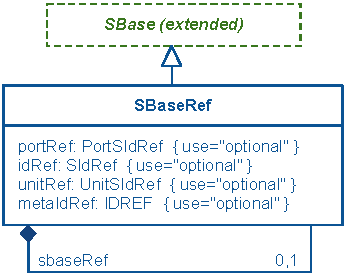
\includegraphics{figs/sbaseref-uml}
  \caption{The extensions of the \SBaseRef class.  The four attributes
    \token{portRef}, \token{idRef}, \token{unitRef} and \token{metaIdRef}
    are mutually exclusive; only one can have a value in a given object
    instance.  The recursive structure also allows referencing entities
    in submodels of submodels, to arbitrary depths, as described in the
    text.}
  \label{sbaseref-uml}
\end{figure}


\subsubsection{The attributes of \class{SBaseRef}}

The four different attributes on \SBaseRef are mutually exclusive: only
one of the attributes can have a value at any given time, and exactly
one must have a value in a given \SBaseRef object instance.  (Note that
this is true of the basic \SBaseRef class; however, derived classes such
as \ReplacedElement may add additional attributes and extend or override
the basic attributes and mechanisms.)

All of the attributes face the following common namespace issue.  As
discussed in more detail in \sec{namespaces}, attributes of type
\primtype{SId}, \primtype{UnitSId}, and \primtype{PortSId} need only be
unique on a per-\Model basis.  This means that an interpreter of the
SBML document must be able to determine the model to which
\token{idRef}, \token{unitRef}, and \token{portRef} attributes refer.
In addition, even though \primtype{ID} values are unique on per-document
level, the same SBML element may be instantiated in multiple submodels,
in any number of \Model objects, and therefore the \token{metaIdRef}
attribute must also know to which \Model instantiation it is referring.
Just exactly how this is done is something that is left up to the
classes that subclass \SBaseRef.  The sections that describe \Port,
\Deletion, \ReplacedElement and \ReplacedBy describe the approach taken
in each case.

Separately, readers may wonder why so many different alternatives are
necessary.  The reason is that in a given scenario, the referenced model
may be located in an external file beyond the direct control of the
modeler, and so the preferred methods of referencing the subobjects may
not be available.  \SBaseRef provides multiple alternatives so that a
variety of modeling scenarios can be supported.

It is also worth noting that classes derived from \SBaseRef may point to
elements from other SBML Level~3 packages.  For example, a package may
define a new \SBase-derived class which will inherit the \token{metaId}
attribute.  These \token{metaId}s may be referenced by the \SBaseRef
\token{metaIdRef} attribute.  Another possibility is that the Level~3
package defines a class having an attribute of the type \token{SId} or
\token{UnitSId}.  In that case, those elements may be referenced with
the \token{idRef} or \token{unitRef} attributes, respectively.  A final
possibility is that the package defines a class with a child element
from the \sbmlthreecore specification (as the Hierarchical Model
Composition package does with Core \Model objects that are children of
the \ListOfModelDefinitions class).  In that case, that child element
may be referenced by any of its identifiers as if it was in its normal
location in \sbmlthreecore.

Because referencing elements in other namespaces is allowed, all classes
that inherit from \SBaseRef must declare what to do when the referenced
element is part of a namespace that the current interpreter does not
understand, and if there are any additional restrictions on referencing
other namespaces.  Any \SBaseRef objects that are not derived classes
defer to their \SBaseRef-derived parent for any such restrictions and
rules.


\paragraph{The \fixttspace\token{portRef} attribute}
\label{sbaseref-portref}

The optional attribute \token{portRef} takes a value of type
\primtype{PortSIdRef}.  As its name implies, this attribute is used to
refer to a port identifier, in the case when the reference being
constructed with the \SBaseRef is intended to refer to a port on a
submodel.  The namespace of the \primtype{PortSIdRef} value is the set
of identifiers of type \primtype{PortSId} defined in the submodel, not
the parent model.


\paragraph{The \fixttspace\token{idRef} attribute}
\label{sbaseref-idref}

The optional attribute \token{idRef} takes a value of type
\primtype{SIdRef}.  As its name implies, this attribute is used to
refer to a regular identifier (i.e., the value of an \token{id}
attribute on some other object), in the case when the reference being
constructed with the \SBaseRef is intended to refer to an object that
does not have a port identifier.  The namespace of the \primtype{SIdRef}
value is the set of identifiers of type \primtype{SId} defined in the
submodel, not the parent model.


\paragraph{The \fixttspace\token{unitRef} attribute}
\label{sbaseref-unitref}

The optional attribute \token{unitRef} takes a value of type
\primtype{UnitSIdRef}.  This attribute is used to refer to the identifier
of a \UnitDefinition object.  The namespace of the \primtype{UnitSIdRef}
value is the set of unit identifiers defined in the submodel, not the
parent model.

Note that even though this attribute is of type \primtype{UnitSIdRef},
the reserved unit identifiers that are defined by SBML Level~3 (see
Section~3.1.10 of the \sbmlthreecore specification) are
\emph{not} permitted as values of \token{unitRef}.  Reserved unit
identifiers may not be replaced or deleted.


\paragraph{The \fixttspace\token{metaIdRef} attribute}
\label{sbaseref-metaidref}

The optional attribute \token{metaIdRef} takes a value of type 
\primtype{IDREF}.  This attribute is used to refer to a \token{metaid}
attribute value on some other object, in the case when the reference
being constructed with the \SBaseRef is intended to refer to an object
that does not have a port identifier.  The namespace of the \primtype{metaIdRef}
value is the entire document in which the referenced model resides, but
must refer to a subelement of the referenced model.  Since meta identifiers are
optional attributes of \SBase, all SBML objects have the potential to
have a meta identifier value.


\subsubsection{Recursive \class{SBaseRef} structures}
\label{sbaseref-recursive-sbaseref}

An \SBaseRef object may have up to one subcomponent named
\token{sBaseRef}, of type \SBaseRef (see \fig{sbaseref-uml}).  This
permits recursive structures to be constructed so that
objects inside submodels can be referenced.

The form of such recursive references must be as follows.  The
highest-level \SBaseRef object of such a chain (which will necessarily
be an object of class \Port, \Deletion, \ReplacedElement or \ReplacedBy,
because they are the only classes derived from the class \SBaseRef) must
refer to a \Submodel object in the containing model.  All child
\SBaseRef objects in the chain must refer to components inside the
\Model instance to which the \Submodel refers.

The following example may help clarify this.  Suppose that we want to
delete an object with the identifier \val{p1} inside the \Submodel
object identified as \val{sub\_m1}.  \fig{submodel-uml} shows that \Deletion
objects are placed inside a \ListOfDeletions within a \Submodel.  The 
following XML fragment illustrates how the constructs will look:

\begin{example}
<submodel id="sub_m1" modelRef="m1">
  <listOfDeletions>
    <deletion idRef="p1" />
  </listOfDeletions>
</submodel>
\end{example}

Suppose instead that the submodel \val{m1} from the previous example is
actually nested inside another submodel \val{m2}.  Then, we would have
the following:

\begin{example}
<listOfModelDefinitions>
  <modelDefinition id="m1">
    <listOfParameters>
      <parameter id="p1" value="3"/>
    </listOfParameters>
  </modelDefinition>
  <modelDefinition id="m2">
    <listOfSubmodels>
      <submodel id="sub_m1" modelRef="m1"/>
    </listOfSubmodels>    
  </modelDefinition>
  <modelDefinition id="m3">
    <listOfSubmodels>
      <submodel id="sub_m2" modelRef="m2">
        <listOfDeletions>
          <deletion idRef="sub_m1">
            <sBaseRef idRef="p1" />
          </deletion>
        </listOfDeletions>
      </submodel>
    </listOfSubmodels>    
</listOfModelDefinitions>
\end{example}

Finally, what if we needed to go further down into nested submodels?
The following example illustrates this:

\begin{example}
<listOfModelDefinitions> 
  <modelDefinition id="m1" name="m1">
    <listOfParameters>
      <parameter id="p1" value="3" constant="true"/>
    </listOfParameters>
  </modelDefinition>
  <modelDefinition id="m2" name="m2">
    <listOfSubmodels>
      <submodel id="sub_m1" modelRef="m1"/>
    </listOfSubmodels>
  </modelDefinition>
  <modelDefinition id="m3" name="m3">
    <listOfSubmodels>
      <submodel id="sub_m2" modelRef="m2"/>
    </listOfSubmodels>
  </modelDefinition>
  <modelDefinition id="m4" name="m4">
    <listOfSubmodels>
      <submodel id="sub_m3" modelRef="m3">
        <listOfDeletions>
          <deletion idRef="sub_m2">
            <sBaseRef idRef="sub_m1">
              <sBaseRef idRef="p1"/>
            </sBaseRef>
          </deletion>
        </listOfDeletions>
      </submodel>
    </listOfSubmodels>
  </modelDefinition>
</listOfModelDefinitions> 
\end{example}


Although this use of nested \SBaseRef objects allows a model to refer to
components buried inside submodels, it is considered inelegant model
design.  It is better to promote any element in a submodel to a local
element if it can be predicted that containing models may need to
reference it.  However, if the submodel is fixed (e.g., if is in an
external file), then no other option may be available except to use
nested references.

\paragraph{Alternate spelling of 'sBaseRef'}
\label{sbaseref-deprecated-spelling}
Because of an error in the UML diagram of a previous version of this specification, a valid spelling of the child \SBaseRef object is the differently-capitalized 'sbaseRef' instead of 'sBaseRef'.  However, this spelling is considered deprecated, and should not be used.  It is expected that future versions of this specification will only allow 'sBaseRef' as the xml name of this object.



% -----------------------------------------------------------------------------
\subsection{Conversion factors}
\label{conversion-factors}

In \sbmlthreecore, units of measurement are optional
information.  Modelers are required to write their models in such a way
that all conversions between units are explicitly incorporated into the
quantities, so that nowhere do units need to be understood and values
implicitly converted before use.  Given the Hierarchical Model
Composition package's design goal of compatibility with existing models
and files that may not be changeable, it is not an option to require
that all included models must be written in such a way that they are
numerically compatible with each other.  For example, if one submodel
defines how a species amount changes in time, and a second submodel
defines an initial assignment for that same species in terms of
concentration, something must be done to make the model as a whole
coherent without editing the submodels directly.  That is the purpose of
the conversion factor attributes on the \ReplacedElement and \Submodel
classes.


\subsubsection{Conversion factors involving \class{ReplacedElement}}

When an element in a submodel has been replaced by an element in a
containing model, old references to the replaced element are replaced by
references to the replacement element.  However, the mathematical
formulas associated with that replaced element may assume different
scales than the ones used for the replacement element.  Correcting this
is the purpose of the \token{conversionFactor} attribute on
\ReplacedElement objects.

There are two types of mathematical references possible in SBML:  assignments
to a variable, and the use of a variable in calculations.  In the former
case, when an assignment (an \InitialAssignment, \EventAssignment, \AssignmentRule,
or \RateRule) targets a replaced element, that formula should be 
multiplied by the conversion factor before being used.  In the latter
case, when a MathML \token{<cn>} element references the replaced element's identifier, that
reference should be considered to be divided by the conversion factor.

For example, if a species has an initial assignment of $4x + 3$, and has
been replaced and given a conversion factor of $c$, the initial assignment formula becomes
$c (4x+3)$.  Conversely, if the $x$ itself has
been replaced by $y$ and given a conversion factor of $c_x$, that initial
assignment formula would become $4((y/c_x)+3)$.  This holds true for any
mathematical equation in the model, including algebraic rules.  This
also means that if a value appears on the right and left-hand sides of
an equation, you must apply the conversion factor twice: if the rate
rule of $x$ is $4x+3$, the rate rule for $y$ becomes $c_x(4(y/c_x) + 3)$.  (This
simplifies to $4y + 3c_x$, as you would expect---the $y$ is already in
the correct scale; it is only the $3$ that must be converted.)



\subsubsection{Conversion factors involving \class{Submodel}}

Most of the math in an SBML model may have arbitrary units, but there
are two exceptions to this rule: time, and reaction extent.  While both
of these mathematical concepts may be scaled to arbitrary units,
multiple such scales in a single document are not allowed: all
references to time assume a single scale, and all reactions are assumed
to process their reactants and products in the same way.  The
\token{timeConversionFactor} and \token{extentConversionFactor}
attributes on \Submodel dictate how time and reaction extent are to be
converted to match the scale of the containing model.  As described in
\sec{submodel-timeconversionfactor}, this includes the MathML csymbols
\token{time} and \token{delay}, as well as any \Delay, \KineticLaw, or
\RateRule objects that are \emph{not} replaced in the \Submodel.

The \token{conversionFactor} attributes on \Species and \Model objects
defined in \sbmlthreecore are unrelated to the conversion factors
discussed above.  The factors in Level~3 Core allow multiple substance
scales to be converted to the (single) scale of reaction extent in a
model, so that different \Species objects may each each have different
units if desired.  Because different \Species objects already have this
mechanism for converting units, there is no need for an additional
\token{substanceConversionFactor} attribute on \Submodel.

To understand the rules, the entire list of classes and MathML elements
that are converted by these three factors (time, extent, and
replaced) in the \sbmlthreecore specification are provided
in \tab{sbml-conversions}.  Similar rules may be derived from other
packages that require any particular mathematics to be universal over 
a given \Model.

\newcommand{\sprd}[2]{\raisebox{-#1pt}[0pt][(#1pt * 2) + 4pt]{#2}}
\newcommand{\persymb}{\emph{Conversion factor for referenced object}}

\begin{table}[bht]
  \rowcolors{2}{sbmlrowgray}{}
  \renewcommand{\arraystretch}{1.175}
  \begin{edtable}{tabular}{p{1.6in}p{2.3in}l}
    \toprule
    \textbf{Component}			& \textbf{Automatic conversion factor}\\
    \midrule
    \AlgebraicRule			& 1\\
    \AssignmentRule			& \persymb\\
    \Compartment			& 1\\
    \Constraint				& \emph{(Boolean value; no conversion factor needed)}\\
    \Delay				& \token{timeConversionFactor}\\
    \EventAssignment			& \persymb\\
    \FunctionDefinition			& 1\\
    \InitialAssignment			& \persymb\\
    \sprd{5}{\KineticLaw} 		& \sprd{5}{$\dfrac{\token{extentConversionFactor}}{\token{timeConversionFactor}}$}\\
    \sprd{5}{MathML \token{<cn>} element} & \sprd{5}{$\dfrac{1}{\textsf{\persymb}}$}\\
    \sprd{5}{MathML \token{<csymbol>} for \emph{time}} & \sprd{5}{$\dfrac{1}{\token{timeConversionFactor}}$}\\
    The time argument to a MathML \token{csymbol} \emph{delay} function & \sprd{5}{\token{timeConversionFactor}}\\
    \Parameter				& 1\\
    \Priority				& 1\\
    \sprd{5}{\RateRule} 		& \sprd{5}{$\dfrac{\textsf{\persymb}}{\token{timeConversionFactor}}$}\\
    \Species 				& 1\\
    \SpeciesReference			& 1\\
    \Trigger				& \emph{(Boolean value; no conversion factor needed)}\\
    \bottomrule
  \end{edtable}
  \caption{Conversion factors used for the different components defined
    by \sbmlthreecore.}
  \label{sbml-conversions}
\end{table}

In \tab{sbml-conversions}, an automatic conversion factor of \val{1}
simply means that the given component does not need to be converted.
Similarly, if a conversion factor is not defined, it defaults to \val{1}
as well.  For example, if the conversion factor
\token{extentConversionFactor} is defined but
\token{timeConversionFactor} is not, kinetic laws are converted
according to the \token{extentConversionFactor}, \emph{divided by~1}.

Note that for the MathML \token{<cn>} element conversion, the
\token{SId} of a \Reaction references its \KineticLaw, meaning that if
the \KineticLaw was converted as per \tab{sbml-conversions}, its
appearance in MathML will also need to be converted by its inverse.  The
identifiers of \AssignmentRule and \RateRule objects cannot appear in
any MathML, and thus do not need to be checked in the same way.

Converting the formula of a \RateRule may involve using a combination of
conversion factors.  If the target of the \RateRule has been replaced
and given a \token{conversionFactor} attribute value, and its \Submodel
has a defined \token{timeConversionFactor} value, the formula must be
multiplied by the \token{conversionFactor} and divided by the
\token{timeConversionFactor} before being used.

There is only one example of math that is assumed to be in the same
scale across a single SBML model but that cannot be converted according
to these conversion factors: the math associated with the \Priority
subcomponent of \Event objects.  When comparing priority expressions
across submodels, they are all assumed to be on the same scale relative
to each other.  Thus, if one submodel had priorities set on a scale of 0
to 10 and another had priorities set on a scale of $-100$ to 100, the
only way to reconcile the two would be to replace all events that had
priorities on one scale with events with priorities on the new scale.
The same would be true of math defined in any other Level~3 package
without the unit type of extent or time, but which was assumed to be
universally consistent across multiple objects in the SBML model.  To
correctly compose models with different scales of such objects using
this package, every nonconformant object would need to be replaced and
given an explicit conversion factor, or that package would have to
extend this Hierarchical Model Composition package to define a new
attribute on the \Submodel class that could be used to automatically
convert all such elements in the submodel with that unit type.


\clearpage

% -----------------------------------------------------------------------------
\subsection{Namespace scoping rules for identifiers}
\label{namespaces}

In the Hierarchical Model Composition package, as in \sbmlthreecore,
the \Model object contains the main components of an
SBML model, such as the species, compartments and reactions.  The
package adds the ability to put \emph{multiple} models inside an SBML
document, and therefore must define the scope of identifiers in such a
way that identifier collisions are prevented.  In this section, we
describe the scoping rules for all of the types and classes defined in
\vrefrange{new-primitive-types}{sbaseref-class}.

\begin{enumerate}

\item A shared namespace exists for \primtype{SId} values defined at the
  level of the SBML document.  This namespace is known as \emph{the
    model namespace} of the document.  It contains the identifiers
  (i.e., values of \token{id} attributes) of all \Model and
  \ExternalModelDefinition objects within the SBML document.  (An
  \ExternalModelDefinition object references a model elsewhere, so in
  this sense, both \Model and \ExternalModelDefinition are types of
  models.)  The namespace is limited to that SBML document, and is not
  shared with any other SBML document, even if that document is
  referenced via an \ExternalModelDefinition.  The identifier of every
  \Model and \ExternalModelDefinition object must be unique across the
  set of all such identifiers in the document.

\item The namespace for \primtype{SId} identifiers defined \emph{within}
  a \Model object used in Hierarchical Model Composition follows the
  same rules as those defined in \sbmlthreecore for plain \Model
  objects.  This namespace is known as the \emph{object namespace} of
  the model.  The scope of the identifiers is limited to the enclosing
  \Model object.  This means that two or more \Model objects in the same
  document may reuse the same object identifiers inside of them; the
  identifiers do not need to be unique at the level of the SBML
  document.  (For example, two model definitions could use the same
  \primtype{SId} value for \Parameter objects within their respective
  contents.  Note, however, that this does \emph{not} imply that the two
  objects are equated with each other!)  An implication of this rule is
  that to fully locate an object, one must know not only the object's
  identifier, but also the identifier of the model in which it is
  located.

\item The identifier of every \UnitDefinition object must be unique
  across the set of all such identifiers in the \Model to which they
  belong.  (This is the same as in \sbmlthreecore.)  This namespace is
  referred to as the \emph{unit namespace} of the model.  Similar to the
  case above, an implication of this rule is that to fully locate a
  user-defined unit definition when there are multiple models in an SBML
  document, one must know not only the unit definition's identifier, but
  also the identifier of the model in which it is located.

\item The Hierarchical Model Composition package defines a new kind of
  component: the \emph{port}, represented by \Port objects.  The
  identifier of every \Port object must be unique across the set of all
  such identifiers in the \Model object to which they belong.  This
  namespace is referred to as the \emph{port namespace} of the model.
  Again, an implication of this rule is that to fully locate a port when
  there are multiple models in an SBML document, one must know not only
  the port's identifier, but also the identifier of the model in which
  it is located.

\item \Reaction objects introduce a local namespace for \LocalParameter
  objects.  This namespace is referred to as the \emph{local namespace}
  of the reaction.  Local parameter objects cannot be referenced from
  outside a given reaction definition.  For the Hierarchical Model
  Composition package, the implication is that the the \SBaseRef class
  (\sec{sbaseref-class}) cannot reference reaction local parameters
  simply by their identifiers (i.e., the value of their \token{id}
  attribute).  However, the \LocalParameter objects \emph{can} be given
  meta identifiers (a value for their \SBase-derived \token{metaid}
  attribute), and be referenced using those.

% FIXME need move this somewhere else:
% 
%   If replaced, it must be by an element in the normal element namespace of
%   a model (such as a global Parameter).  Old references to that replaced
%   LocalParameter will then point to the new replacement element.  If a
%   LocalParameter is deleted from a Reaction whose KineticLaw used it in
%   its math, that KineticLaw may still be valid if there was an element
%   in the element namespace of the model with that same id to which it
%   can now refer (in other words, if the LocalParameter shadowed a global
%   parameter).


\end{enumerate}

The following example may clarify some of these rules.  Suppose a given
SBML document contains a \Model object having the identifier \val{mod1}.
This \Model cannot contain another object with the same identifier
(e.g., it could not have a \Parameter object with the identifier
\val{mod1}), nor can there be any other \Model or
\ExternalModelDefinition object identified as \val{mod1} within the
same SBML document.  The first restriction is simply the regular SBML
rule about uniqueness of identifiers throughout a \Model object; the
second restriction is due to point (1) above.  On the other hand, there
could be a second \Model object in the same document containing a
component (e.g., a \Parameter) with the identifier \val{mod1}.  This
would not conflict with the first \Model identifier (because the
\Parameter would be effectively hidden at a lower level within the
second \Model).

